% ---------------------------------------------------------------------
% -------------- PREAMBLE ---------------------------------------------
% ---------------------------------------------------------------------

%\documentclass[12pt,a4paper,english,oneside]{article}
\documentclass[preprint,authoryear,12pt]{elsarticle}

\usepackage[utf8]{inputenc}
\usepackage[english]{babel}

\usepackage{calc}
\usepackage{natbib}
\usepackage{url}
%\usepackage{listings}
\usepackage{hyphenat}

\usepackage{supertabular,array}
\usepackage{lipsum}
\usepackage{booktabs}
\usepackage{graphicx}


% Strike through
\usepackage[normalem]{ulem}

% Punctuation for references
\bibpunct{[}{]}{;}{n}{,}{,}

% correct bad hyphenation here
\hyphenation{op-tical net-works semi-conduc-tor}


% Multiple bibliographies
%\usepackage{multibib}
%\newcites{gen}{References}
%\usepackage{bibentry}


% ---------------------------------------------------------------------
% -------------- DOCUMENT ---------------------------------------------
% ---------------------------------------------------------------------

\journal{Information and Software Technology}

\begin{document}

% Extra definitions?
\selectlanguage{english}

\begin{frontmatter}

%% use the tnoteref command within \title for footnotes;
%% use the tnotetext command for the associated footnote;
%% use the fnref command within \author or \address for footnotes;
%% use the fntext command for the associated footnote;
%% use the corref command within \author for corresponding author footnotes;
%% use the cortext command for the associated footnote;
%% use the ead command for the email address,
%% and the form \ead[url] for the home page:
%%
%% \title{Title\tnoteref{label1}}
%% \tnotetext[label1]{}
%% \author{Name\corref{cor1}\fnref{label2}}
%% \ead{email address}
%% \ead[url]{home page}
%% \fntext[label2]{}
%% \cortext[cor1]{}
%% \address{Address\fnref{label3}}
%% \fntext[label3]{}

%% use optional labels to link authors explicitly to addresses:
%% \author[label1,label2]{<author name>}
%% \address[label1]{<address>}
%% \address[label2]{<address>}

\title{Adopting agile in the large: motivations, success factors and challenges}

\author{Kim Dikert}
\ead{kim-karol.dikert@aalto.fi}

\author{Maria Paasivaara}
\ead{maria.paasivaara@aalto.fi}

\author{Casper Lassenius}
\ead{casper.lassenius@aalto.fi}

\address{Aalto University, School of Science, Department of Computer Science and Engineering}


% ---------------------------------------------------------------------
% ------------------------- ABSTRACT ----------------------------------
% ---------------------------------------------------------------------

\begin{abstract}

Agile methods have become an appealing alternative for companies striving to
improve their performance, but the methods are originally designed for small and
individual teams. This poses challenges when introducing agile to large
organizations where development teams can not be autonomous. We reviewed 30
experience reports and case studies describing the process of taking agile
methods into use in large organizations. The primary motive for agile adoption
is the need to improve performance. For a successful transformation the entire
organization must be aligned and all organizational units must participate.
Creating an agile community in the organization will help the change to stick.
Typical problems are misunderstanding of the agile model, and difficulties
coordinating multiple agile teams.

\end{abstract}

\begin{keyword}
%% keywords here, in the form: keyword \sep keyword
%% MSC codes here, in the form: \MSC code \sep code
%% or \MSC[2008] code \sep code (2000 is the default)

agile \sep transformation \sep large scale \sep adopting agile

\end{keyword}

\end{frontmatter}


% ---------------------------------------------------------------------
% --------------------------- TEXT ------------------------------------
% ---------------------------------------------------------------------


\section{Introduction}

--> Introductory paragraph

--> Motivation for research
-- There are no systematic reviews for this
-- A collection of experience reports can be used for creating a theoretical
   base.
--> There is interest in large scale [ref XP13 workshop]

--> Freudenberg, S. and Sharp, H., "The Top 10 Burning Research Questions from
    Practitioners," IEEE Software, pp. 8-9, 2010.

--> Why is large scale software development different from smaller scale?

--> This literature review is intended for researchers as a theroretical
   and proven foundation for the real problems that organizations face in
   transformations.
   This is also intended to be directly usable by practicioners, to serve as a
   base of general advice with strong motivation (although every organization
   has unique needs).


% ---------------------------------------------------------------------
\section{Background}
\label{sec:background}

Lindvall, M., et al., "Agile Software Development in Large Organizations,"
IEEE Computer, vol. 37, pp. 26-34, 2004.


Boehm, B. and Turner, R., Balancing Agility and Discipline: A Guide for the
Perplexed: Addison-Wesley, 2003.
Boehm, B., "Get ready for agile methods, with care," IEEE Computer, vol. 35,
pp. 64 - 69, 2002.
--> Any hints on size?? Maybe size leaning towards discipline?


% ---------------------------------------------------------------------
\section{Research method}
\label{sec:method}

The goal of the research was to aggregate evidence on how large organizations
transform into an agile way of working. The research was conducted as a
systematic litterature review based on empirical studies.

\subsection{Research questions}

The following research questions were set to guide the research process.

\begin{itemize}

\item
RQ1: Why do large organizations initiate an agile transformation?

\item
RQ2: How do large scale agile transformations usually proceed; do
     transformations exhibit patterns?

\item
RQ3: What are typical successes and challenges in a large scale agile
     transformation process?

\end{itemize}


\subsection{Definition of large scale}
\label{sec:largescale}

A key question in the study was the definition of \emph{large scale}. Large
scale requires additional coordination and makes communication difficult
compared to software development in small teams.

--> Needs to have complexity in software design?? --> What is complexity in software?
    Is ``complexity'' an issue in agile?
    What will bring complexity into software? Not costs or the length of the
    schedule. --> Having many people will bring the complexity in terms of the
    SDM to use.
--> Some people see cost as a definition for large scale, some see code base
    size [Petersen], some see project duration [Bjarnson?]. These are all
    related, but do not relate to any specific problem. You can spend X amount
    of money, but it does not in itself make any difference if the money is
    spent in an agile way.
--> Formal definitions (EU, etc.) look at project costs or company turnover.
    These definitions do not take a standpoint on complexity of the product, so
    they do not matter in the context of SDMs.

--> Ref: the XP conference
--> [Cockburn 2003] Agile is best suitable for teams around 50 people or fewer.
--> Boehm, B. and Turner, R., Balancing Agility and Discipline: A Guide for the
    Perplexed: Addison-Wesley, 2003. --> There might be a 50 person boundary?
    --> See Boehm also for list of 

--> The company must already be with N teams or N people, not growing up to the
    required numbers. Small companies in growth are therefore excluded. 


\subsection{Research process}

The research was conducted as an application of Kitchenham's
\cite{Kitchenham2007} guidelines for systematic literature review. The selection
of primary studies was done as a keyword based database search and manual
filtering of included studies. The filtering process was executed independently
by two researchers (Dikert, Paasivaara). The selected primary studies were coded
for data extraction and analysis. The entire process was audited and mentored by
a third researcher (Lassenius).

We deviated from Kitchenham's guideline on the part of data extraction. Instead
of using data extraction forms we analyzed the primary studies by coding. This
deviation was made in order to minimize how possible preconceptions would affect
the data extraction step, and to use a specialized software tool that allowed us
to record evidence in as much detail as possible.
% --> Possibility to find many different viewpoinits for the research questions
% --> Lots of items, which would have lead to much diversity in data extraction form 

\subsubsection{Inclusion criteria}
\label{sec:inclusioncriteria}

Based on the research questions and intended focus of the research, we defined
three facets to guide inclusion/exclusion decisions: agile software engineering,
focus on transformation, and large scale. The first facet covers primary studies
focusing on software engineering organizations applying or striving to apply
agile methods. The second facet states that included studies must provide
insights relevant to organizational transformation, and specifically to the
research questions. The third facet underlines the particular contribution we
aim to provide with this research, namely the exclusive focus on large
organizations. These three facets were used for inclusion and exclusion in each
study selection step, including search string design, filtering by abstracts,
and full text filtering.

Examples on topics excluded by the first facet are agile manufacturing, and
applying Scrum practices in management boards, as these do not relate to
software engineering. In addition, we required that the organizational
transformation was aimed to introduce agile methods, which excluded other
development methods than agile \cite{Sagesser2013}, and use of agile
methods in other contexts than software development \cite{Hodgkins2007}.

The facet of \emph{organizational transformation} was interpreted so that the
primary study must present insights on the process of transformation. This
was the most important facet, as the pivot of this research is to examine
how the transformations happen. Examples on excluded topics are comparing the
original and agile development methods \cite{Petersen2010}, discussing use of
agile in a large organization but not describing how the new methods were
introduced \cite{Mishra2011}, and merely presenting agile tools in large scale
use \cite{Kim2012}. These sources were excluded as they did not privide insights
on organizational transformation.
% Also [Fitzgerald 2005] on just presenting use of agile methods, no introducing

Transformation and ``scaling up'' are very closely related and in some cases
they are one and the same. For instance, if transformation begins with a pilot
and spreads gradually through the organization, the process can very well be
seen as a ``scaling up'' journey. However, we excluded cases where a initially
small organization was scaled up \cite{Maranzato2012}, and discussions with a
process centered viewpoint without describing organizational change
\cite{Lyon2008}.
% Also [Greening 2010] on process centered viewpoint without transformation

The facet of \emph{large scale} was interpreted as presented in section
\ref{sec:largescale}, having 50 development personel or 6 teams as as the limit
for large scale. In some cases the source presented very vague indicators on
size. For instance, we deemed the case presented by Cloke \cite{Cloke2007} to be
included as there was indications of large scale considerations, although the
size remained unclear. The case presented by Miller and Haddad \cite{Miller2012}
was deemed to be excluded as there was no indications whatsoever on size. A
borderline exclude was the case presented by Tudor \cite{Tudor2006} as there was
no indication of issues indicating large size, althoug there were several
development teams.
To complicate matters, some papers talked about ``the team'' in singular when
referring to the organization \cite{Hodgkins2007}, making it clearly nontrivial
to judge whether an organization was large based on the choice of words of the
author.

A further example on exclusion by the \emph{large scale} facet were cases with
large organizations but only a single team adopting agile \cite{Fulgham2011}.
We considered cases of single teams (although in large organizations) unrelated
to this research as our focus is on transformation of the entire organization.
Also piloting cases that resulted only in single teams using agile were excluded
\cite{Scott2008}.

% Also [Jensen 2003] with only a single team
% Possibly [Mc Cormic 2005] on single team piloting

In addition to the criteria listed above we excluded studies that were not
empirical. We excluded textbooks, studies merely presenting theories, and other
studies that did not include any case organization. We also excluded studies of
benefits or limitations of agile in general. Lastly, we excluded student
experiments as it is implausible to simulate the dynamics of a large
organization in an experiment.


\subsubsection{Preliminary searches}

% --> Why are the preliminary searches done?

Before proceeding with the database search a number of preliminary searches were
performed. The purpose of the preliminary searches was to create a benchmark of
potentially relevant papers that should be matched by the actual database
search. We also wanted to list top ranked hits by trivial keywords that the
more complex final search string might miss. Initial searches were made using
keywords that were as general as possible, including ``agile transformation''
and ``large scale agile''. Additionally, a trial keyword search was done in the
selected databases (listed in table \ref{table:databases}) using the following
search string:

\begin{verbatim}
((agil* OR scrum OR xp OR lean) AND
(transform* OR transit* OR change OR migrat*) AND
((large AND (scale OR organization))) OR enterprise)
\end{verbatim}

From these preliminary searches we compiled a list of 117 possibly relevant
papers that should be matched by the actual database search.

\subsubsection{Study selection}

The study selection process inlcuded three steps, each step refining the set of
selected papers. First a database search was used to gather an initial set of
papers. This set was then refined by filtering out abstracts and finally full
text filtering. The study selection process is outlined in Figure
\ref{fig:selectionprocess}.

\begin{figure}[b]
  \begin{center}
    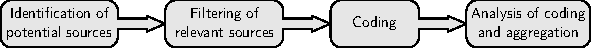
\includegraphics[width=1\textwidth]{graphics/research_process.pdf}
    \caption{Study selection process}
    \label{fig:selectionprocess}
  \end{center}
\end{figure}

A keyword search in online databases was chosen as the means to find potential
primary studies. The databases included in the search are listed in Table
\ref{table:databases}. All databases supported use of complex boolean logic in
searches which allowed us flexibility when constructing the search strings.

\begin{table}
    \begin{tabular}{ p{0.28\textwidth} l l }
        \toprule
        Database         & URL                         & N of matches   \\
        \midrule
        IEEExplore       & http://ieeexplore.ieee.org      & 745 \\ 
        ACM              & http://dl.acm.org               & 168 \\
        Scopus           & http://www.scopus.com/home.url  & 1596 \\
        Web of Knowledge & http://apps.webofknowledge.com  & 786 \\
        \bottomrule
    \end{tabular}
    \caption{Databases included in search, and number of matched articles}
    \label{table:databases}
\end{table}

We constructed a search string based on the facets \emph{agile software
deveolpment} and \emph{organizational transformation}, as presented in section
\ref{sec:inclusioncriteria}. Preliminary searches had showed that picking
keywords with good precision was difficult. Therefore we decided to exclude the
facet \emph{large scale} from the keyword search, with the consequence of
increasing the manual filtering effort in the subsequent steps.
Having a substantial part of the matches in non-relevant areas such as agile
manufacturing, we included only articles including the term ``software'' or
articles published in relevant conferences. Instead of engineering the search
terms any further, which proved to result in excluding some relevant articles,
we chose to rely more on manual filtering. The resulting facets and keywords are
listed in Table \ref{table:searchterms}.

\begin{table}
    \begin{tabular}{ p{0.22\textwidth} p{0.76\textwidth} }
        \toprule
        Facet                  & Keywords   \\
        \midrule
        Agile methods\newline (before \& after) &
            \texttt{agile, scrum, "extreme programming",
            waterfall, "plan-driven", RUP}\\
        Organizational transformation &
            \texttt{transform*, transiti*, migrat*, journey, adopt*, deploy, introduc*,
            "roll-out", rollout}\\
        Only software\newline related atricles &
            \texttt{(software OR (conference="agile, xp, icgse, icse"))
            AND NOT (title+abs="manufacturing" OR conference="agile manufacturing")}
        \\
        \bottomrule
    \end{tabular}
    \caption{Facets and related search terms used}
    \label{table:searchterms}
\end{table}

The database keyword search matched 1874 unique papers. The abstracts of these
papers were categorized independently by both Dikert and Paasivaara into three
categories: include, excude, and uncertain. The result was combined by marking
abstracts both researchers agreed on for inclusion or exclusion respecitvely.
The inclusion of disagreed or uncertain abstracts was resolved through
discussion. At this stage papers were excluded only if both reserachers deemed
it clearly irrelevant, including any uncertain cases for full text filtering. As
a result 170 papers were selected for full text filtering.

We also evaluated the keyword search against the benchmark created in the
preliminary search step, concluding that 75 of the 117 preliminarily selected
papers matched. The missed 32 preliminary papers were examined, resulting in
including 3 additional papers as primary sources.

% Inter-rater statistics
%
%                     Maria
%            excl   ???   incl    TOT
%      excl  1578    18    15    1611
% Kimi ???     84    17     8     109
%      incl    51    42    62     155
%      TOT   1713    77    85    1875
%
% ???'s =  169
% in/ex = 1706
%
% Pr(Kimi, in) = in / (tot)  =  155 / 1857 = 0.0619
% Pr(Kimi, ex) = ex / (tot)  = 1611 / 1857 = 0.8675
% Pr(Maria, in) = in / (tot) =   85 / 1857 = 0.0458
% Pr(Maria, ex) = ex / (tot) = 1713 / 1857 = 0.9225
%
% Pr(e) = Pr(Kimi, in) * Pr(Maria, in) + Pr(Kimi, ex) * Pr(Maria, ex) = 0.8031
%
% Pr(a) = (ex-ex + in-in) / tot = 0.8831
%
% k = 0.4063

Full text filtering was performed by evaluating each article against the three
facets of the inclusion criteria. Filtering was done in two steps. In the first
step Dikert extracted data relevant to the three facets of the inclusion
criteria. Based on the extracted data 76 papers could be immediately deemed as
included or excluded. The remaining 94 papers were evaluated against the
inclusion criteria by both Dikert and Paasivaara, and a decision was made after
discussing each paper separately. In difficult cases Lassenius was consulted to
reach a decision. As a result of the full text filtering 47 papers were selected
to be included.

In the full text filtering step the references of all papers were also examined
for relevance, including 2 referenced papers as primary sources. Most case study
papers used references very scarcely, mostly referencing well known descriptions
of agile methods.

Finally, counting 47 papers from the full text filtering step, 3 papers from
preliminary searches, and 2 papers from references, 52 papers were selected
as primary studies.

In several cases there were more than one primary study presenting the
transformation of the same organization. Even if the transformation of a single
organization was described in many studies all sources that passed the inclusion
criterial were included. Studies presenting the same organization were treated
as one unit so that we could gain as much insight from each organization as
possible. There were also a few papers that presented multiple case studies, and
in those cases we treated each studied organization individually. As a result 42
unique organizations were identified in the primary studies. We use the term
\emph{study} to refer to the primary study publications, and the term
\emph{case} to refer to an individual case organization that may be described in
several different studies.

% -----------------------

% - pitää olla systemaattinen
% - pitää olla toistettava
% ==> Perustuu enimmäkseen siihen että on 2 tutkijaa toistamassa
% 
% Jos koko on epäselvä:
% --> Tutkijat päättävät keskustelun ja kvalitatiivisen harkinnan perusteella
% --> Tähän tarvitaan esimerkit, milloin on otettu mukaan, milloin on karsittu
%     pois


\subsubsection{Study quality assessment}

The primary research for this literature review consists almost exclusively of
industry experience reports. This may be seen as a factor lessening the
evidence.
--> Why did we do this anyway?
--> Case studies with research method studying organizational transformations in
    software industry are very scarce.
--> Large organizational changes are hard to measure experimentally (controlled
    experiments?). Also due to this any student research was excluded.

The reason for deviating stydy assessment
--> Original research consisted almost solely of experience reports
--> The fact that experience reports have a subjective standpoint makes it
    unreliable to make quantitative conclusions based on the data
--> We also decided to include separate studies describing the same organization.
    This was useful as it deepened the understanding of each case, and several
    large organizations have produced more than one description of their agile
    transformation.

The fact that the study is based on a quantitative basis
--> Experie reports have a subjective bias
--> The data synthesis must not rely on quantitative measures. This means that
    we also considered topics raised by only a marginal number of reports.
--> It may still be interesting to make some quantitative observations such as
    a particular problem being reported in the majority of reports.

It was quite common that a single transformation case was described by many
papers. For example, one paper would highlight the viewpoint of developers
\cite{Fry2007}, and another would consider the transformation from user
experience designers' point of view \cite{Federoff2009}. Instead of using the
most complete paper as suggested by Kitchenham \cite{Kitchenham2007}, we
combined the results presented in each paper and considered the case as a single
unit. By doing this we avoided bias caused by duplicate publications, and were
enabled to have a more detailed view of the case organization.


\subsubsection{Coding of primary documents}

The primary documents were coded using the Atlas TI qualitative data analysis software.
An integrated deductive and inductive approach was chosen for coding the primary
studies \cite{Cruzes2011a}. The coding was designed to have a contextual part
and a findings part as also suggested by Cruzes and Dybå \cite{Cruzes2011a}. A
list of codes was established for contextual information, as presented in Table
\ref{table:contextualcodes}. Codes related to the research questions were chosen
to be created by an inductive process. The reason for inducting codes rather
than using an a priori approach was to avoid the researchers' previous
assumptions of the research area to affect the choice of codes

\begin{table}[h]
    \begin{tabular}{ p{0.28\textwidth} p{0.7\textwidth} }
        \toprule
        Contextual code     & Explanation   \\
        \midrule

Agile method & Agile methods used in the organization (eg. Scrum, XP) \\

Business area & The business area in which the organization operates. \\

Organization size & Mentioning the size of the case organization. \\

Time of\newline transformation & When the transformation has been in
progress, or how long the transformation has taken. Possibly relative to
the time of the research. \\

Research process & The paper describes a research process. \\

Geographical\newline location & Where the organization is located. \\

Large scale definition & A definition of "large scale" software development. \\

Multisite / GSD & Mentioning of a multisite organization. \\

        \bottomrule
    \end{tabular}
    \caption{Context information}
    \label{table:contextualcodes}
\end{table}

To give direction for code induction seven different code families were
established, as presented in Table \ref{table:codefamilies}. A description
defining scope and examples for codes were defined for each family. The example
codes would not necessarily be used as actual codes, and would not represent the
entire or final scope of the families.

\begin{table}[h]
    \begin{tabular}{ p{0.32\textwidth} p{0.65\textwidth} }
        \toprule
        Code family          &  Description
        \\
        \midrule

        RQ1: Reason to change &
        Reasons to start the transformation (demand for faster delivery). \\

		RQ2: Transformation\newline process &
		Statements that describe the transformation process (top-down, big bang,
		stepwise). \\

		RQ3: Challenges &
		Statements that present challenges in the transformation (change resistance).
		\\

		RQ3: Success factors &
		Statements that present success factors in the transformation (management
		support).
		\\

		Investing in change  &
		Factors that present how the organization is investing in the
		transformation (training, consultants, tools). \\

		Practices &
		Distinguishable practices that are used or established during transformation.
		Factors that are presented as neutral in terms of successes and challenges
		in the primary studies.
		(coaching, piloting, continuous integration, communities of practice) \\
		
		Contextual &
		Contextual codes defined in Table \ref{table:contextualcodes}. \\
		
        \bottomrule
    \end{tabular}
    \caption{Code families}
    \label{table:codefamilies}
\end{table}

The inductive coding was done according to the guidelines described below.

A passage of text that presents any concept relating to the research questions
or the contextual codes becomes a quotation. If the quotation corresponds
closely to a concept that has already been coded the existing code is used.
Otherwise a new code is created, and the code is assigned to one of the
predefined code families. The labels of existing codes may need to be adjusted
when new quotations are assigned. Many codes may be assigned to one quotation
and quotations of different codes may be overlapping.

The length of the text passage that make up a quotation may vary. For the
contextual codes the quoted passage should be of minimal length. For other
quotes the length of the quotation should be long enough to highlight the
context of the concept the quotation, varying from a few sentences to one
paragraph, or even several paragraphs. As an example of context of the
quotation, if a transformation challenge is described by a quotation it would be
good if also the source or resolution of the challenge could be included in the
quoted text passage. Having enough context should broaden the understanding
of the coded concept when looking at the quotation in isolation..

% -- Considering that mentioning the inclusion of a factor as a success, then
%    would the absence of the same factor be a challenge?

The total accumulated codes and quotations of the integrated deductive and
inductive coding process are presented in Table \ref{table:codecount}. The total
number of quotations is less than the sum of quotations in the categories
because a single quotation may have multiple codes.

\begin{table}[h]
    \begin{tabular}{ l r r }
        \toprule
        Code family    &  Codes  &  Quotations
        \\
        \midrule
        RQ1: Reason to change &        30 &  123 \\
		RQ2: Transformation process &  16 &  580 \\
		RQ3: Challenges &              40 &  323 \\
		RQ3: Success factors &         44 &  260 \\
		Investing in change  &          5 &  137 \\
		Practices &                    11 &  170 \\
		Contextual &                    8 &  215 \\
		Total &                       154 & 1575 \\
        \bottomrule
    \end{tabular}
    \caption{Number of codes and quotations per code family}
    \label{table:codecount}
\end{table}


\subsubsection{Validation of coding}

Coding was done by only one researcher due to resource constraints and volume of
source material. As recommended by Kitchenham \cite{Kitchenham2007} we conducted
an experiment with the goal to assess the consistency of coding that two
independent researchers may achieve.
In the experiment Dikert and Paasivaara coded independently a sample of five
primary documents. The sample was hand picked as a representative subset of the
source material. The coding was done relying solely on the guidelines presented
in the previous chapter, and the researchers were careful not to discuss the
choice of codes or interpretations relating to codes before the experiment was
completed. Finally the independent codings of the two researchers were analyzed
with two metrics: by the number of matching themes found, and by the amount of
overlap in quotations similar codes have.
% See Kitcenham, chapter 6.4

The metric of matching themes measures how well the independent researchers are
able to induct similar codes from the source material. As codes are inducted it
is likely that two researchers label similar quotes differently. To overcome
this problem we defined higher level themes under which the individual codes
were organized. Through discussion we made decisions on whether differently
labeled codes could be organized under the same theme or not. Table
\ref{table:codingexperiment} presents the total number of themes the researchers
found in each document, and how many of the themes were matching. We concluded
that on average two of three themes found by one researcher are similarly found
by the other researcher, but one of three themes is not found by the other
researcher.

The metric of quotation overlap measures how well the quotations for similar
codes match between two independent researchers. The intent is to measure how
codes that are deemed similar by their names match in the actual quoted text. On
a scale of 0 to 3 we evaluated the quoted text of codes in each theme that
matched for both researchers, as described in the previous paragraph. A score of
3 was given for matching codes whose quotation content was virtually the same
for both researchers. A score of 2 was given if the quotations were mostly the
same, but other researcher had included one text passage that the other had
missed. A score of 1 was given if roughly half of the quotations were the same.
If the quotations had less similarity than this a score of 0 was given. One code
provided typically 1 to 3 quotations per document. The quotation overlap score
was counted including only codes that had matching themes. We concluded that the
average quotation overlap score was 2.2.

\begin{table}
    \begin{tabular}{ l r r r }
        \toprule
        Document    &  Matching themes  &  Total themes  &  Quotation overlap (0-3) \\
        \midrule
        P1          &  14  &  19   &  2.1  \\
        P2          &   6  &  11   &  2.4  \\
        P3          &   7  &  11   &  2.1  \\
        P4          &   2  &   4   &  2.3  \\
        P5          &  12  &  16   &  2.0  \\
        \bottomrule
    \end{tabular}
    \caption{Result of independent coding experiment}
    \label{table:codingexperiment}
\end{table}

Combining the quotation overlap result and the result that inductive coding
yielded similar themes with a factor of two thirds, we conclude that two
different researchers should agree completely on at least half of the quotations
in the source material of our study. This agreement includes both that the
researchers select the same text passage as a quotation, and that researchers
agree with the meaning of the quotation. Further interpretation of the
quotations and codes will still remain a subjective matter.


\subsection{Limitations of research method}

-- A keyword search can not identify the facet of \emph{large scale}, and also
   \emph{transformation} is difficult to capture with keywords. Because of this
   we assume that it is likely that a some studies have been missed by the
   keyword search. As an improvement we would suggest combining the entire
   archive of \emph{Agile Conference} and \emph{Agile Processes in Software
   Engineering and Extreme Programming} to the results of the keyword search.
   These two conferences provided more than two thirds of the pimary sources.

-- Few of the primary studies presented a research method. Most of the studies
   were experience reports where the author was a member of the organization
   discussed. Because of this we must assume that the primary studies are
   biased. Due to this risk of bias we chose not to make statistical
   interpretations of the results. We only use relative measure when comparing
   results.

-- We avoid numbers in results, such as frequency of a phenomena, except in the
   meta-analysis section.

% ---------------------------------------------------------------------
\section{Results}
\label{sec:results}

This section presents the findings of the literature review. In the first
subsection a meta analysis of the analyzed papers is presented. In the
subsequent sections findings are presented organized according to the research
questions. The methods used for extracting the results were described in section
\ref{sec:method}. Note that the term \emph{study} is used when refering to a
primary study publication, and the term \emph{case} is used when refering to an
organization which may be described in several studies.

\subsection{Overview of primary studies}

The results of this study include findings from 52 primary studies presenting
how 42 different large software organizations introduce agile methods. Most of
the included studies were experience reports (45 studies), and in many cases it
was evident that the author had been personally involved in the transformation.
Only 6 of the included studies had a research method explicitly stated. One of
the studies was an interview article. The publication forums of the primary
studies were distributed so that 57 sources were conference proceedings, 4
sources were journal articles, and one source was a technical report.

\begin{figure}[b]
  \begin{center}
    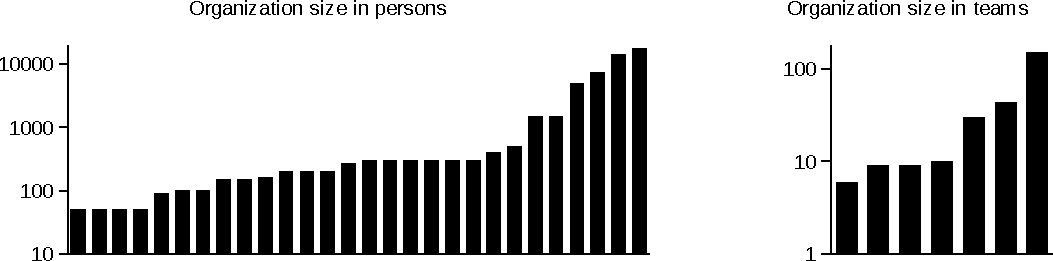
\includegraphics[width=1\textwidth]{graphics/organization_size.pdf}
    \caption{Distribution of organization sizes in primary studies}
    \label{fig:organization_size}
  \end{center}
\end{figure}

The size of the organizations varied from the minimum included size of 50 to
18,000 people. The median size was 300 people. In 7 studies the size was
presented in terms of teams, ranging from the minimum of 6 teams to 150 teams.
The median was 10 teams. In 8 studies there was no direct indication on size
but the issues discussed revealed that the organization was of large size
accoding to our definition. The distribution of organization sizes is presented
in figure \ref{fig:organization_size}.

Figure \ref{fig:transformation_time} summarizes the publication years of the
primary studies, and the years when the transformations were reported to have
started. All studies and transformations were dated after year 2000. There were
peaks in transformation studies in years 2008 and 2011. The studies were
typically published two years after the start of the transformation.

\begin{figure}[t]
  \begin{center}
    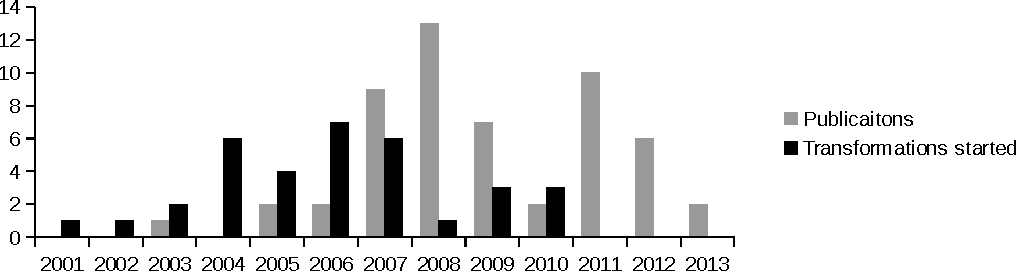
\includegraphics[width=1\textwidth]{graphics/transformation_time.pdf}
    \caption{Publication years and reported start years of transformations}
    \label{fig:transformation_time}
  \end{center}
\end{figure}

\begin{table}[bh]
    \begin{tabular}{ l r }
        \toprule
        Business area    &  Case organizations   \\
        \midrule
		Online services for consumers and business  &  9  \\
		Telecommunications                          &  7  \\
		Enterprise management                       &  5  \\
		Banking and financial services              &  4  \\
		Healthcare                                  &  3  \\
		IT services                                 &  2  \\
		Government                                  &  1  \\
		Information security                        &  1  \\
		Not specified                               & 10  \\
        \midrule
		Total                                       & 42  \\
        \bottomrule
    \end{tabular}
    \caption{Business areas of case organizations in primary studies}
    \label{table:businessareas}
\end{table}

The business areas of the case organizations are presented in table
\ref{table:businessareas}. Different business areas were represented somewhat
evenly. Online services was the largest group, including companies
providing software as a service solutions for businesses, online media players
for consumers, online services for consumers, and communication software for
businesses. The second largest group was telecommunications, including companies
such as British Telecom, Cisco, Ericsson, and Nokia Siemens Networks. The third
largest group was enterprise management solution providers with products for
business process management, project protfolio management, and facility
management.


\subsection{Agile methods used}

The agile methods reported being used in the transformed organizations are
summarized in table \ref{table:agilemethods}. The most prevalent method was
Scrum, which was the sole agile method mentioned in 25 cases. The second most
mentioned agile method was Extreme Programming (XP). Lean software development
was mentioned in some studies, although combined to Scrum in all cases. Other
agile methods mentioned were Unified Process, ADM, and Rapid Application
Development. In one case the agile method was not named.

It was quite common that organizations sought to combine agile methods.
Especially Scrum, XP, and Lean software development were used together. In
addition, many cases mentioned use of XP practices without explicitly stating XP
as the process being used (such as test driven development and continuous
integration). Combining and customizing agile practices was also evident in that
many organizations viewed the agile method as continuously evolving.
Organizations evolved the agile methods for instance through retrospectives and
continuous improvement.

\begin{table}[t]
    \begin{tabular}{ l r }
        \toprule
        Method                             &  N  \\
        \midrule
        Scrum                              &  25 \\
        XP                                 &  4  \\
        Scrum and XP                       &  5  \\
        Other                              &  4  \\
        Combining Lean to an agile method  &  6  \\
        Not specified                      &  1  \\
        \bottomrule
    \end{tabular}
    \caption{Agile methods reported in number of cases}
    \label{table:agilemethods}
\end{table}

\subsection{Reasons to change}

As stated by Research Question 1 we investigated the reasons organizations start
a transformation process towards agile software development. Most primary
studies mentioned reasons for starting the transformation, and only 7 cases of
42 did not mention any reasons. In the cases giving no specific reason to change
it was simply mentioned that management had decided to change the organization.
The identified reasons for organizations to change are presented in table
\ref{table:reasonstochange}.


% Some cases reported that the organization had been successful in waterfall
% delivery for a long time before the agile transformation.


\begin{table}
    \begin{tabular}{ p{1.2cm} p{1.2cm} l }
        \toprule
        \multicolumn{3}{l}{Reasons to change}  \\
        \midrule
        
        \multicolumn{3}{l}{External issues: Need to respond to changes in business}  \\
        
        &  \multicolumn{2}{l}{Demand for more frequent deliveries} \\
        &  &  Time To Market must lessen  \\
        &  &  Long cycle times are seen as problematic  \\
        
        &  \multicolumn{2}{l}{Something must be done in order to remain competitive} \\
        &  &  Change is required to stay in business  \\
        
        &  \multicolumn{2}{l}{Customers demand improvement} \\
        
        &  \multicolumn{2}{l}{Demand for flexibility or responsiveness} \\
        &  &  Demand to accomodate changes efficiently  \\
        &  &  Better responsiveness to customer requests  \\
        
        
        \multicolumn{3}{l}{\rule{0pt}{4ex} Internal issues: Problems in managing software development}  \\
        
        &  \multicolumn{2}{l}{General problems with management of software development} \\
        &  &  Management dysfunction  \\
        &  &  Problems with motivation and morale  \\
        &  &  Problems coordinating a growing organization  \\
        
        &  \multicolumn{2}{l}{Problems with overhead and excess in process}  \\
        &  &  Excess, slowness and costs caused by process  \\
        &  &  The current process is being ignored  \\
        
        &  \multicolumn{2}{l}{Problems with planning or keeping schedules}  \\

        &  \multicolumn{2}{l}{Too long cycle time before feedback}  \\
        
        &  \multicolumn{2}{l}{Demand to improve product quality}  \\
        
        
        \multicolumn{3}{l}{\rule{0pt}{4ex} Communication and collaboration issues}  \\
        
        &  \multicolumn{2}{l}{Communication and collaboration dificulties}  \\
        &  &  Problems in communication across and within projects  \\
        &  &  Teams work in silos or isolation  \\
        
        &  \multicolumn{2}{l}{Requirements engineering issues}  \\
        &  &  Requirements are not understood  \\
        &  &  Unawareness of what is important  \\
        
        &  \multicolumn{2}{l}{Demand of better customer collaboration}  \\
        
        \bottomrule
    \end{tabular}
    \caption{Summarizing why large organizations initiate an agile transformation (RQ1).
             The table presents a hierarchial view of reasons for the organization to change.}
    \label{table:reasonstochange}
\end{table}

The reasons to change were are grouped in three top-level categories: external
issues, internal issues, and communication issues. External issues are related
to the business area which the organization is operating in. Internal issues are
related to the way the organization is managed and software is being developed.
Communication and collaboration issues are related to internal and external
collaboration. Change was motivated by known problems in these categories, such
as known process dysfunctions or communication problems. There was also internal
and external demand for improvement, for instance in speed of delivery and
quality.

\subsubsection{External issues}

The most prominent reason for introducing agile methods was the demand to
deliver software faster and more frequently. A common statement was that it was
necessary to reduce the Time To Market (TTM) [P17, P18, P32, P39, P47]. As
stated in one study: ``The market was moving faster than the development group
was able to deliver'' [P38]. Long cycle time, i.e. time from start of project to
delivery, was seen as a problem in itself [P25, P36]. Some studies indicated
that the organizations set as one of the transformation goals to deliver
software faster [P2, P8]. Other cases described that development was generally
considered as slow [P36, P46, P49].

Commercial competition and market situation was seen as a trigger for
transformation. Especially speed of delivery was seen as a means to respond to
the competition [P9, P38]. As Greening describes: ``The average release duration
peaked at 41 and 35 months, an alarming state that could enable competitors to
gain market share.'' [P19]. In many cases the transformation was seen as
essential for the company to remain competitive [P10, P11, P18, P42, P49]. For
instance, British Telecom realized that ``From a strategic view, there is little
alternative than to change the old ways of working'' [P32].

Demands for change and improvement were also expressed by internal and external
customers. Again, the requests of the customers reflected the need of faster
development and release cycles [P5, P39]. As described in one study: ``Speed of
delivery is of the essence – customers are no longer prepared to wait for 18
months or more for solutions to be delivered'' [P23]. In some cases business
partners expressed mistrust in the original way of conducting development [P40,
P46].

Yet another frequent external factor driving for improvement was the need to
accomodate change during development. Organizations saw agile as a opportunity
to improve responsiveness to change in general [P25, P26, P42].
Some organizations faced difficulties when changes to plans were needed. For
instance, the organizational struture made adapting to changes difficult [52],
and making changes created management overhead [P51]. Other organizations saw an
business advantage if priorities could be changed as required [P8, P39].
Customers and business representatives were in many cases attributed as the
sources of change requests, and the responsiveness to customer requests needed
to be improved [P18, P33, P36, P49].

\subsubsection{Internal issues}

The internal issues relate to how software development is managed in the
organization. In many organizations the project management practice was in a
state of dysfunction, and it needed to be corrected. Management problems were
for instance constantly recurring crisis events [P30], managers ignoring
prioritization of tasks [P38], and reluctance towards focusing on delivering
business value [P49]. Some cases stated that projects simply failed [P21]. Some
organizations wanted to improve generic project management practice, such as
risk management [P8], management of offshoring [P38], and improving the quality
of life of team members [P44]. Several organizations were growing and
experienced that the old development method did not scale up [P16, P30, P50, P51].
There was also a desire to improve team motivation and commitment, and
collaboration between management and developers [P39].

Command and control style management where ``a few people, usually those
farthest from the action, made the decisions without directly involving the
developers doing the actual work'' was highlighted as a problem [P44]. For
instance, schedules could be dictated by management, and teams had to comply to
them regardless of the workload [P9]. As a result teams were overworked and
needed stretch far to finish projects on time. Low morale and motivation were
identified as problems that needed to be fixed, and agile was seen as a solution
[P25, P30, P40].

A common problem that was acknowledged in organizations was overhead in process,
which showed as bureucracy and needless costs. Examples on overhead in process
were unproductive meetings [P38], sign-offs and gates [P9], excessive focus on
conformance to process [P40], and change management overhead [P51]. Creating
excessive documentation instead of business value was seen as a problem in some
cases [P24, P35].
From business representatives point of view the processes were unreasonably
costly, while at the same time insufficiently capable of delivering business
value [P36, P46, P49]. In one case business realized that customers did not
request the heavy CMMI based process [P24].
A heavy process resulted often in ignoring the process, only paying ``lip
service'' to the process, or applying its steps retroactively [P6, P9, P49].
Seffernick described how applying the waterfall process had teams ``still
developing the same old way but slower because of the additional process''
[P46].

A slow process with long cycle times leading to late feedback was a problem in
the old model. A large investment was required before results were visible [P5],
and there was variances in expectations and what was delivered [P40]. A related
problem was late integration which caused extra work [P25]. As organizations
grew and products became more complex test cycles began to lengthen, which
hindered flexibility and reduced speed [P33, P50].

Yet another problem in managing development was problems with schedules.
Some cases described schedules as unpredictable and estimation being difficult
[P16, P30, P40, P51]. In other cases it was reported that release deadlines were
often missed [P19, P21, P33, P41].

Finally, the original process model was seen as a cause for quality problems.
Several studies mentioned a demand for better quality, and quality improvement
was set as a goal for the agile transformation [P25, P31, P41, P42]. Improvement
in external quality and customer satisfaction were also anticipated from agile
development [P2, P4]. Problems with technical debt were attributed to the
original process. Some cases reported on prioritizing new feature development
over bugfixes or fixing only the easiest issues [P30, P38].


\subsubsection{Communication and collaboration issues}

Many organizations experienced problems in communication and collaboration
between projects, teams, and even members of a single team [P38, P21].
Teams were in many cases organized around components and were working in silos.
Working in silos diluted focus and made adapting to change difficult, as teams
could only focus on their limited area of expertise [P7]. Functional silos acted
against creating a shared purpose in operating [P40], and resulted in a ``ball
over the wall'' mentality [P46]. Distance between teams was also created by
document driven communication, and was causing misunderstanding of requirements
[P24].

Other communication issues were related to requirements handling and difficulty
to focus on the most important aspects of a delivery.
Examples on problems with requirements was too much focus on the documenting
aspect instead of providing understanding [P24, P49], and ignoring the fact that
requirements and understanding are evolving during a project [P4].
In some cases the organization of work and management was such that it hindered
focusing the development [P7], and prioritization of what to work on was not
done efficiently [P38, P39].

Too little customer and user collaboration led to problems in some
organizations. For instance, too late user involvment led to change requests
late in the project [P40]. There was a wish to collaborate more frequently and
in less formal ways [P4, P26].


A few organizations were experiencing rise of agile methods at grass roots
level, but the agile teams could not collaborate efficiently with other parts of
a waterfall organization. Tensions arose when teams using different development
approaches attempted to work together on products [P10]. On a team level agile
had enabled some flexibility, but that flexibility could not be leveraged on the
scale of the entire organization [P26]. This kind of experiences drove the
organization to deploy agile on a full scale.


\subsection{Transformation process}

\subsubsection{The initial state of the organization}

We investigated the initial state of the case organizations before the
transformation. The typical initial process model was described as waterfall, as
stated in 25 cases. In several cases the authors characterized the initial state
of the organization as ``traditional''. CMMI was presented as a driver for the
original process in 4 cases. Other process models the studies named were RUP
[P19], Prince2 [P51], and Macroscope [P14]. In 9 cases the initial state was not
described.

The old model was described in most cases briefly and in a neutral sentiment.
Waterfall development in general was referred to as ``traditional, plan-based
methods'' [P25], ``traditional phase-based approach'' [P36], or ``old fashioned
process driven waterfall'' [P23]. Korhonen [P25] referred to the model presented
by Royce \cite{Royce1970} when describing the initial state.

In some cases specifics of the old model was criticized. The characteristics of
the old process models were described as having ``many gates and sign-offs
required by upper levels of management'' [P9], ``lot of bureaucracy in project
management and a strict hierarchy of requirements communication'' [P39], and
``project managers typically used a command-and-control philosophy'' [P44].

In a few cases the initial process model was less rigid, and closer to the agile
model that was to be introduced. Examples of such loose process models were
described: ``The choice of development methodology is one of any number of
degrees of freedom granted to teams at Amazon. Development teams are expected to
solve their problems in the best way possible'' [P3], ``the R\&D group leveraged
a loose, waterfall-based process with an entrepreneurial culture'' [P16]. Some
organizations had even signs of agile development on team level although the
surrounding organization operated in a waterfall fashion. This was described as
``Agile and Scrum were increasingly popular and emerging at a grass-roots level,
at a corporate level Yahoo! still embraced a more traditional product
development process'' [P10], and ``some teams had applied scrum on the team
level, despite the surrounding organization that was working with a waterfall
software engineering model'' [P26].

In a few cases the organization initailly lacked strict process. For instance
Long describes the initial state in the following way: ``Project scope was in
constant flux. Well-meaning market and product owners routinely inserted new
requirements during product development.'' [P30].

Some authors describe the developement being originally organized in silos. For
instance Ranganath describes that ``Teams operated in silos. Collaboration,
shared purpose and ownership for outcomes were hard to find'' [P40].


\subsubsection{Modes of transformation}

Work in progress...

Top down

Bottom up

Big bang

Transitional


\subsection{Challenges in transformation}

Any organizational transformation involving numerous individuals will face some
challenges. As stated by Research Question 3, we investigated what are typical
challenges that large organizations introducing agile methods face.

Challenges can be organized on a high level into three categories. First we
discuss challenges relating to managing the transformation. These challenges
relate to managing people and resourcing. Secondly we present challenges in
choosing and establishing a suitable agile model. Thirdly challenges related to
large organization size are presented. Size will bring challenges such as
coordinating work between many teams and adapting other functions than
development to agile.



\subsubsection{Change resistance}

To start a transformation the organization needs an initial push. However,
people are usually disincluned to change, and it is likely that resistance
will emerge in any change. 
% Change resistance is a central challenge in any organizational transformation.
People will not be willing to change unless there are good reasons, and the
change is preceived easy enough. It is difficult to attain a buy-in for a
change, and even organizations that have a flexible culture will face resistance
[P10]. It should be expected that not everyone will be willing to change, and
some employees will never adapt to the change [P6]. In one case it was reported
that objections from team members was a major reason for loss in time and
productivity [P29].

On a team level numoerous reasons for change resistance were given. For
instance, Fecarotta described the organization of Boeing as risk-averse and
cautious which slows down any change [P14]. The organization was also described
having a deeply rooted status-quo because of high employee retention, which
further hindered change. In some cases it was reported that people worried about
new roles and responsibilities that agile would possibly bring [P44]. For
instance, testers were worried that they would need to take on cross functional
tasks, which would be outside their area of expertise [P18]. Yet another reason
for change resistance was the move from own offices to team areas [P22]. People
were also feeling being monitored because of the increased level of interaction
within the team and between project stakeholders [P45]. One study reported the
cultural change required for middle management as the biggest cause of
resistance [P2].

In these cases change resistance was mitigated for instance by education [P45],
and one-to-one discussions [P22]. Change resistance was also softened by using
first only teams willing to try agile, so that insights could be gathered to
ease the continued transformation [P45].

Another common form of change resistance that was reported was skepticism.
Seffernick describes how management did on one hand acknowledge benefits of
agile, but on the other explained away the possibilitiy to apply it due to
contract reasons, the current matrix organization, and other organizational
practices [P46]. In that case the director of development still pushed the agile
transformation forward. Skepticism was often created by other similar
misconceptions, including that agile does not work for complex products [P5,
P36], agile needs to be implemented in a prescriptive by-the-book way [P9], that
frequent meetings will cause overhead [P18], and that agile equals avoiding
governance and working without a plan [P8].

% For instance, teams may not be willing to try
% new approaches unless they have been proven [P6]. 

% Resistance is to be expected --> there are many different stakeholders [P41]

% * No value seen by some groups, e.g. mainframe or maintenance [P49]

The way the transformation is initiated will also affect how change resistance
will show.
In many cases the initiative to change came from management, but when presented
wrong the initiative becomes a mandate that pepole are not receptive for. Spayd
[P49] summarizes this as: ``Organizations do not change merely because the boss
says so, at least not in the way that is intended''. In that organization the
introduction of CMM had been carried out consistently by a mandate, but the
collaborative nature of agile did not mix well with such a mindset. A top down
mandate may also dilute the understanding of the reasons for starting the
transformation, and the understanding of agile development overall [P2].
O'Connor describes how team members became sceptical towards agile when
implementing mandaetd changes did not bring any visible benefits [P37].

Organizations had also bad experiences if the implementation of the agile model
was prescribed. For instance, doing Scrum based on checklists of practices would
not work [P41]. Benefield described that it was challenging to find a balance
between independence for teams to choose their way and diluting the value and
structure of Scrum [P6]. Giving room for team autonomy is one of the critical
facets of agile, but it must be ensured that teams do not discard practices that
add value and structure.

The problem of tension between management and development may also be opposite.
In cases where the change was emerging bottom up the reluctancy to change was
not in the team members but management. This caused that significant
organizational change could not be raised above the team level.
For instance, Atlas [P3] describes how it would have required executive support
to integrate the product management office and separate quality assurance groups
in the agile process. In this case, when managers owning projects with many
teams were not involved in the transformation, the agile model was restrained
from spreading beyond team level. Lack of middle management support was also
seen as the most serious shortcoming by Spayd [P49]. Middle management is in a
position to undermine the entire transformation, and may do so if they do not
participate in, and thus understand, the agile method. Agile brings changes to
some management roles [P2], and lack of understanding of agile development will
leave managers feeling left out [P6]. Still one problem is that if management
does not speak out a goal towards using agile, developers feel that the agile
methods may be replaced by something else at any time [P12].

\subsubsection{Other organizational issues}

% Lack of plans (a guess -- not included)?

% Agile zealots

Another issue that should be avoided is overenthusiasm towards agile methods.
In several cases there was mentionings about change leaders or teams becoming
agile zealots. For instance, Evans describes how some members of the agile
community were becoming too evangelic, which made people take sides for or
against agile development [12]. In another case team members started out with an
overly eager attitude, but when agile did not deliver improvements the
interest faded and started to go back to the old process [P20]. Attempting to
implement agile too strictly may cause conflicts, and especially in a large
organization the change leaders need to maintain a collaborative attitude
towards various groups in the surrounding organization [P6]. Introducing agile
methods does not guarantee success, and therefore they should not be followed
blindly [P4].

% People do not speak their minds

In one case a passive-aggressive organization culture was described as a
challenge. Ranganath describes how people did not speak their minds in meetings,
thus creating a false sense of agreement when talking about how the organization
should develop. Because of this resistance and concerns were left growing, and
acted against achieving a successful transformation. To to avoid these issues
change leaders worked with team members on an individual level to win confidence 
and make their voices heard [P40].

% Old work and commitments, schedule pressure

A condition hindering the transformation was that old commitments still needed
to be tended to even though the organization was being restructured.
Some organizations started their agile journey in a state where people were
overcommitted, but it was later realized that overloaded people will not be able
to learn new ways of working and changing their behavior [P37, P42]. Cowan [P11]
describes how time was allocated for tending to old commitments. However, even
when there was preparation for extra work people with specific expertise became
overloaded. After time it was realized that overcommitment must be reduced by
allowing to shift excess work for later time [P11]. In another case management
forced people to remain committed to firm deadlines, even midst in the
organizational transformation. The engagement in old commitments and tasks
resulted in ignoring new practices introduced by agile, and eventually the agile
method was breaking down [P21]. Spayd [P49] also describes how senior management 
pressed teams to deliver what the customer had been promised, regardless of what
the current velocity of development predicted.

% Physical spaces, challenge of finding a seating

In some cases the old way of working had people seated physically distributed,
in opposite to what agile methods typically suggest. Office spaces needed to be
arranged so that the entire team could work in a single room, but it took time
and effort, and it was not always possible [P36, P6]. Lewis and Neher describe
how dedicated rooms for teams could not be arranged, and team events such as
daily standups required booking a conference room [P29]. In another case the
estate organization shut down the teams' attempts to modify working spaces
[P49].

% Lack of training and coaching 

Lack of resources allocated for supporting a transformation was an evident
problem. Resources were most often short for training and coaching, but
underbudgeting these activities may be a serious mistake.
Hajjdiab [P20] describes how reluctance of management to invest in training
caused teams to be ill prepared for the agile transformation effort, and
eventually resulted in ending the use of agile methods. As a less dramatic
outcome of shortened training was lower motivation [P45].

Proper coaching was a particular problem for very large organizations. In cases
where the number of teams in need of coaching was large the demand often
exceeded the capacity of available coaches [P1, P6, P23, P49]. Lack of coaching
was also attributed as a reason why the success of pilot teams could not be
repeated when agile was adopted more widely [P9, P45].
Silva and Doss [P47] described that when it was hard to fill the coaching
positions people less seasoned in agile were appointed as coaches, which risked
that agile practices would not be taught correctly.

% Add quote?
% * No coaching --> Applying techniques improperly --> Damage
% [P9]
% Without proper coaching however, the success of these informal teams met with
% mixed results over the longer term.  In retrospect, many of these teams did
% damage to themselves by improperly applying Agile techniques, particularly when
% command and control mechanisms were still in place.


\subsubsection{Falling back to old model}

In several cases challenges in the transformation resulted in people falling
back to the old model of working.
In some cases it was only a struggle to learn agile practices, but in other
cases the old model displaced agile.
Development work has to go on during the transformation but there will be new
things to learn for the team. Stress caused by the combination of schedule
pressure and much change at once will pull people back to the old way of working
[P11, P18, P38].
Schatz and Abdelshafi tell how even subtle trouble may risk the transformation,
as people will always look for reasons to revert to familiar behavior [P44].
Teams without adequate training were struggling with applying agile practices
correctly, and the challenge the new practices posed made people to abandon them
and return to the ways they know [P6, P49]. 

In some cases agile was seen as an overhead, and was therefore abandoned. For
instance, as new practices were being introduced there was a decrease
performance, and when teams realized that the benefits are not immediate they
started reverting to the old model [P21].

When a release schedule with fixed deadlines that business required was combined
to agile managers started to behave authoritatively and the self organization of
agile started to break down [P31]. % (Skeptics used this as a sign of that agile can not work)

In one case new senior appointments were changed the management to be less
favorable towards agile, and a waterfall development model started to return
[P12].

% Include quotation?
% * Some teams mirrored waterfall approaches in their behavior --> Did not work
% [P32]
% Then comes execution and the learning really begins. Teams’ working habits
% determine their success.  Often teams quickly ignore plans in favor of using
% tactical approaches that mirror waterfall thinking. This contrasts nicely with
% those more attuned to applying agile.


\subsubsection{Agile is found to be hard}

A challenge most organizations came across was that an agile model was difficult
implement. An experienced software team may do well in training, but when the
time comes to apply agile techniques in practice the team may get lost [P21].
Agile was also seen as a solution to all problems [P9], success was declared
prematurely [P49], and expectations created by successful early experiments were
not fullfilled [P38]. Disapointment was granted when these hopes were not
fullfilled and implementing an agile model was found to be hard and time
consuming. The difficulty in implementing agile is evident in misconceptions of
the agile model, when by-the-book implementations prove to be insufficient, and
when the agile methods were applied badly to the organization.

% Misconceptions of agile

There were many examples on problems caused by misconceptions of what agile
software development is. On a general level, Bang [P4] describes how the values
of the agile manifesto were not understood, and agile practices were carried out
without understanding their purpose. In one case management saw the purpose of
agile simply being faster product delivery [P9].

On a team level there were several examples of misunderstanding the agile model.
Cases describe how agile was seen as freedom to hack without documentation
[P26], that development could be done without design tasks [P37], and that agile
meant that everyone should become a generalist [P42]. Schatz and Abdelshafi
describe how teams presented unfinished work at reviews and ignored the
principle of showing only completed increments, which resulted in a backlog of
bugs [P44]. In one case team members had perceived the introduction of agile as
a means to squeeze out more efficiency [P45]. In addition, the flatter
organization was seen as fewer career opportunities, and pushed team members to
internal competition for visibility [P45].
Still one misunderstanding of agile was due to perceiving it only through the
tools used, such as project management software [P48]. Superficial focusing only
on tools themselves and not the reasons behind their use led to frustration
[P42].

In some cases the misunderstanding of the agile model was described as ``doing
mini waterfalls'' [P6]. Managers were using Scrum terminology, but at the same
time committing unreasonable workloads on teams [P6]. In another case a
waterfall nature was seen in giving task estimates as hours left, and task
breakdowns disconnected from what was really being done [P27].

% By the book is not good

Even if there was no misunderstandings the correct agile model was found hard to
implement. Several cases describe how an agile model was hard to learn from
literature [P21, P27], especially when it comes to implementing it on a large
scale [P13]. As Beavers [P5] writes: ``There simply was not a manual or document
where we could find easy answers on how to do things''.
Schnitter and Mackert [P45] report that theoretical considerations on how to
scale up the agile methos were not good enough, and that product managers and
architects struggled when several Scrum teams were working concurrently.
Another case concluded that all practices prescribd in XP did not fit enterprise
scale development, and some practices required customization [P49]. It would not
be good to prescribe practices with a check list as it would impose a single
model in an organization with several individual teams and projects [P41].

Further indications were given that the advice given in literature will not
ferry all the way. Benefield [P6] describes how it was dificult finding a
balance between prescribing a by-the-book implementation which may put people
off, and giving too much freedom in the agile methods which may weaken core
practices.
The reality where the practices needed to be applied was described as
messy in comparison to the ideal circumstances presented in literature, which
made it difficult to choose an initial model and gain buy-in for it [P10].
Difficulties in choosing the model to start with were also due to variances
perceived in the agile approaches suggested in literature [P30].

% Customizing badly (mapping to old model)

The difficulty of agile and misunderstandings were also evident in cases where
the methods were customized badly. As by-the-book implementation often was not
feasible the agile method was tailored to suit the needs of the organization.
However, in some cases tailoring meant skipping some practices, which lead into
problems. In one case certain individuals were allowed to ignore some core
elements of Scrum, which came to turn the teams decision making into a variant
of command and control [P9].
Lewis and Neher [P29] describe how there was temptation to strip some practices
and enhance others. Previous attempts had proven that one of the reasons early
attempts of agile had failed was deviations from the process, because of which
the agile mindset did not take root [P29]. In a bad implementation customization
may lead to the team taking only practices that reflect their current needs, and
therefore failing to achieve a real change in process and mindset [P9, P46].
Another example of bad customization that counteracts change is replacing agile
vocabulary in favor of familiar terminology from the old model, because
introducing new language will also create new ways of thinking [P44].


\subsubsection{Large organization issues}

% The software produced in a large organization may have size and complexity that
% agile struggles to handle.

The primary studies revealed challenges on two areas which relate particularly
to large scale. First, a large software development endeavour must handle
integrating the work products of many teams. Second, a large organization will
have management challenges not seen on small scale.



% Coordinating between many teams

%% ?? -->
% Include this ???
% Large organization put agile methods under the test of scaling up, and problems
% were encountered. One case reported use of agile across hundreds of teams, but
% management could not get a roll up of the progress without having strict rules
% on how status was reported [P48]. Schnitter and Mackert [P45] report that a
% maximum workable size in a project managed by Scrum was 130 people including 7
% development teams.


Many cases reported that introducing agile practices soon yielded improvements
on the team level, but as a part of a large transformation teams needed to
change their external behavior also.
The initial success was followed by challenges when teams needed to work with
other teams and as parts of the larger surrounding orgaization [P13, P17, P24].
Introducing agile had created flexibility on a team level, but it could not be
fully utilized as the surrounding organization was not responsive enough [P26].
There were dependencies between teams in the agile model as well, and the
dependencies made managing development difficult [P9, P10].

In the agile model it was hard for managers to get an overview of the progress
of the release [P17]. The status of features was hard to tell because different
aspects of features were sepatated across teams [P17]. Smits and Rilliet [P48]
report that providing executive overview of the development programs was limited
by the tools used to manage agile projects.

Some organizations attempted to initially create a model where teams operate
autonomously, which is well in line with agile principles. However, a number of
issues arose from independence. For instance, teams had to balance between the
team's own goals and broader goals of the entire organization, and some teams
chose focus on their own goal [P7]. Coordination was obstructed by independent
teams that did not respect the larger context they were working in [P13].
Coordination was also difficult when different teams were working for different
customers but the applications being built were interdependent [P29]. One case
reported that allowing teams to have different sprint durations created delays
in delivery [P51].

Also technical problems relating to inter-team coordination were reported.
Integrating the products of teams was seen as a problem in some cases [P5, P50],
and lack of standardized build scripts was mentioned as a problem in one case
[P27].
There was also problems in synchronizing definitions of software interfaces
between teams, and dependencies in code caused problems in larger features
[P26].
One case reported that team centricity in the agile model created a fragile
architecture, divergence in coding style, and even distrust between teams [P24].

Further problems were encountered when scaling up agile over many sites.
Operating in a distributed environment makes communication more difficult, which
causes problems with agile when frequent and effective communication needs to be
achieved. Distribution had negative effects, such as missing kick-off meetings,
reduced feeling of proximity when telecommunication is necessary, and difficulty
in arranging frequent meetings due to time zone differences [P45].
Agile project management was also problematic in a distributed setting. In a
waterfall model separate parts of projects could be isolated to different sites,
but the agile model does not allow such strict slicing of projects [P29].
In one case it was simply admitted that a distributed organization will impose
additional burden on communication and require additional care in the process,
but distribution and agile would still be used together [P48].

Moore and Spens [P34] describe the progression of the above mentioned
coordination problems. At first cross-team dependencies were attempted to be
reduced, but it became evident that the dependencies were an inherent part of
the project. A traditional approach to managing dependencies created excess
work, reduced independence and flexibility of teams, and created contract based
and adversarial relationships within the organization. There was some success
when up to 5 teams were coordinated using Scrum-of-Scrums, but that model could
not be scaled to a global level. The main problem was teams that were thinking
too much inside the team walls. When the new practices were scaled up the
communication channels narrowed and created communication breakdowns. Problems
with collaboration, dependencies, and integration were solved with presnce of
individuals with an proactive and open mindset towards working over team
boundaries. It was concluded that a balance is needed between completing new
stories from the team backlog and maintaining overall stability of the
application. [P34]

Many studies presented solutions for the inter-team challenges, which also
highlight the challenges themselves. The general model of solving inter-team
problems was introducing an additional layer of coordination, such as a
Scrum-of-Scrums team [P43], a similar product team [P45], or an entire
customized release framework [P13]. In one case integration problems were
controlled by prioritizing code quality and maintaining existing functionality
over new features [P13]. Finally, the choice of tools was reported to have an
impact on the coordination effort [P17].



% Challenge: Previous organization in silos is haunting new model
% Is this good??

In some cases problems were caused by internal boundaries or silos in the
initial organization. Cloke [P10] describes how use of Scrum revealed an
internal segmentation where teams operated with differing priorities and
agendas. This segmentation also hampered the initial effort to use Scrum in a
larger context [P10].
Projects needed specialized skills that were scarce and people were often
relocated to match the needs of the moment, but too much reorganization made
it diffucult for teams to plan ahead [P11].
A dispersed matrix organization causes also problems when people are on one hand
kept assigned to many projects simultaneously, but on the other hand functions
such as database administration, architecture boards, and project management are
centralized [P14].


% Challenge: Differing vocabularies

In a large environment many agile teams coexist and it is possible that their
agile models and vocabularies start diverging. When many teams implement agile
without consistent guidance friction and fragmentation may be generated [P9].
The organization may require moving people between teams from time to time, and
therefore it would be desirable that no big differences in teams' agile cultures
exist. Divergence in process would create risk increasing costs when relocating
people [P38]. Further, if processes of teams diverged management had
difficulties in forecasting and comparing work of different teams [P38, P48].
To overcome problems with divergence in agile models some organizations defined
standards to follow [P8, P43].

% Roles of managers

A common problem in the agile implementations was the role of managers.
Especially the role of middle management was seen as unclear in agile
methods, but a cultural change would still be required on that level [P2].
It was described that people in management positions needed to resist the
tendency to take command and control to allow room for self-organization, but
the change in role was difficult to achieve for the people involved [P11, P52].
Nielsen and McMunn [P30] describe how the project management group had
previously worked through big up front plans and competing of resources, but
those ways would need to dramatically change.

% Roles of managers (continued)

Several other problems related to management roles were also presented. For
instance, Spayd [P49] describes how managers were left outside the roles offered
by the new agile model. In another case when Scrum masters were appointed from
the ranks of managers developers felt being micromanaged because of vague
understanding of the agile method [P27]. It was also described how mixing the
role of project manager and Scrum master created a conflict in interest, and
turned the Scrum manager's role into one of policing the team instead of
supporting the team [P30]. In some cases problems with manager positions were
solved by phasing out roles relating to the old model, and replacing them with
new positions more suitable for agile [P38, P52].

% Using two models side by side
% Part of the organization is in old mindset

In most cases a large organizational transformation proceeded gradually, and
during the process it was possible that the new agile model was used in parallel
with the old methods. The arrangement of using the old and new models side by
side was seen as problematic [P1, P26], and causing tensions on all organizational
levels [P10]. Ongoing projects had been set up with previous development
methods, and the agile methods had to be arranged to fit with them [P8, P29].
A particular problem in sychronizing work between projects using different
models was that in Scrum the software design was fleshed out over time as
sprints progressed, but the waterfall model would require detailed design to be
locked early in the project [P29].

Despite the agile introduction there were problems with management working
according to the old waterfall model. O'Connor [P38] described management as
``focused on meetings and big up front project plans'' despite agile being in
use. In another case management was losing confidence in agile because familiar
reports on cost analysis and percentage complete were not produced [P35]. As
Scrum teams did not commit to fixed schedules they were considered unreliable
according to the original model [P45].

There were also problems with duplicating management when two models were in
effect. For instance, agile teams were required to comply with current
procedures producing excess documentation and stepping through approval gates
[P20, P21]. The bureucracy of the previous traditional model was still enforced,
and management was not convinced to lighten the process. Another case describes
that after introducing the agile method teams were required to fill in templates
of two processes [P48].

% Add quote ?
% * Especially higher organizational levels were not using agile --> Problem
% [P3]
% Scrum still exists mostly in a way that avoids conflict with the larger
% corporate organization, and there has been little progress in addressing larger,
% organizational impediments.

% [P18]
% Real Agile teams will experience resistance when they start working with
% non-Agile interfaces. Lack of understanding in ‘why to help create a cadence?’,
% ‘why involve the customer more?’ will cause resistance in the change process.

% --> ``Part is in the old mindset''
% * Problem: Management attempts to use a ``resource pool'' of individuals rather than coordinating teams
% [P6]
% we face the constant threat that restructuring and the instinct from management
% to track and leverage resources at the individual level (for example
% organization-wide resource pools) will destroy the team dynamic and adversely
% affect productivity.


\subsubsection{Integrating other functions than development to agile}


Agile methods are typically understood through a set of activities closely
related to software development. Cases describe how development teams were
typically the first entities in the organization that were considered when
introducing agile [P2, P17, P31, P38]. However, development operates in a larger
context, and will need to interface with other organizational functions.
Challenges were faced when exposing other parts of the organization to the agile
mode, and functions that were further away from development were resistant to
change [P2, P18, P31]. A tension was growing between development and broader
roles in the organization [P1]. The full beenfits of the transformation would
not be attained unless the entire organization was set to work along the same
paradigm [P18, P42].

Primary sources listed various functions beyond development that are involved in
bringing products to the market. Marketing was a particularly frequently
mentioned group [P5, P17, P28, P31, P38, P45, P48]. Other groups involved in the
whole of product delivery were sales [P17, P31], infrastructure and operations
[P10, P45, P46, P50], user experience and design [P9, P10, P28], documentation
[P28], legal [P10], security [P10], customer services [P48], and finance [P48].
All of these groups were reported to be affected on some level by the agile
transformation.
% separate QA [P3], --> Later human resources --> Later

Agile affects timings in the software delivery lifecycle which caused two types
of problems. Firstly, the iterativeness of agile models was problematic when
interfacing with other functions. Iterativeness changed the pace of delivery
[P17], and forced design to focus on a shorter scope [P15]. Various groups
feeding and supporting development had earlier committed once to a long term
plan, but in the new arrangement they needed to adjust to incremental delivery
[P48].

Federoff and Courage [P15] describe how the user experience team struggled with
the 

--> Iterativeness and UED

--> DS + UED [P6, P9, P10, P15+P28]


The second type of problems was that some release activities would inevitably
have a long lead time, such as acquiring export clearances and licensing
authority. A particular function that required extended periods of stability was
sales and marketing, as they were required to make customer commitments and
communicate upcomming releases a relatively long time ahead. [P31]
[P38] --> See marketing lead time?


The increased delivery speed of development teams caused infrastructure and
operations teams to fall behind, and they were forced to update their way of
working [P46, P50].


Some cases reported that development efforts were controlled on a top level by a
project management office (PMO). The PMO was described as entrenched in a
waterfall paradigm, and the top-level rigidity was causing friction in the
agile adoption [P3, P6]. The PMO was seen as a hub and bottleneck controlling
all aspects of projects, and its central structure had to be dismantled for
the organization to become agile [P46].

Problems in adopting agile were even showing in functions outside the software
delivery lifecycle. A support function that was particularly mentioned to
have issues in agile adoption was human resouces (HR).


%%%%%%%%%%%%%%%%%%%%%%%%%%%


UED

* Problem: Idea of iterative design was not welcomed by user experience experts, interaction designers and visual designers
* These groups would have preferred designing up front
[P6]
Design is made up of user experience experts, interaction designers and visual
designers. The designers’ initial reaction to Agile was similar to the way
engineering architects react when faced with the idea that you don’t design
everything up front, that you constantly refactor, and that requirements will
change. They were quite taken aback.


* Problem: user experience specialists need to keep the big picture within iterations
[P9]
the user experience specialists’ main difficulty was how to keep the entire user
interface design in perspective, and still iterate on specific components.
Comment: The UX people were considered part of the team.


* Problems: Interaction with some groups caused blocking issues
* User Experience and Design, operations, legal, and security team
[P10]
CROSS-FUNCTIONAL DEPENDENCIES: However well we did within the team, we also
frequently ran into dependencies on other groups often in other locations –
groups such as UED (User Experience and Design), operations, legal and the
Yahoo! security team (affectionately called the Paranoids) – which were
identified as blocking issues but almost never neatly resolved within our sprint
boundaries.




"C: Adapting non-development parts of organization to agile"


SOME KIND OF GENERAL ADJUSTMENT?

* Challenge: Product teams need to communicate with business management
* Challenge: Communicating with marketing
* Challenge: Field services
* The ways of working had to be changed for these groups
[P45]
Upscaling methods were mainly driven by theoretical considerations. Implementing
them revealed that the skills and knowledge of product managers and software
architects were often not sufficient to manage a number of Scrum teams
concurrently. Product teams had to communicate with business management,
marketing, and field services who were not fully prepared for how Scrum and the
product teams’ expectations would change their daily work. The process of
software requirements engineering were found to require a major adjustment.


ITERATIVENESS / SPEEDED UP INCREMENTAL DELIVERY

* Problem: Development started with agile --> Other departments needed to adapt to iterative delivery
* Challenge: Product manager --> rethink definition of releases
* Challenge: Marketing --> Adjust how products are taken to market
* Challenge: Sales --> Manage customer expectations --> Frequency of new functionality
* Challenge: How to make commitments to customers --> Requirement priorities
[P17]
Like many organizations, BMC’s decision to adopt Agile practices started in the
development organization. These changes inevitably impact the rest of the
company as all departments adapt to this new pace of incremental value delivery.
Product managers must re-think how they define releases and work with
development. Marketing must adjust how it takes products to market. Sales must
reset customer expectations on how frequently they have access to new
functionality.
As they gain experience with agile, BMC is changing the way they make
commitments to customers. Discussions with customers are centered more on
requirement priorities and how those priorities can be delivered earlier and
with greater satisfaction.


* Challenge: Surrounding organization adaption
* Internal customers --> manufacturing, customer services, marketing, sales, field and partner enablement, training, demos, documentation, finance
* Problem: They were not familiar with incremental planning --> Originally they committed once
[P48]
We have found, though, that the most difficult part of our transition is getting
everything else that must feed and support the product development teams in
place. In the past, supporting and surrounding organizations counted on having a
content commitment once. From this, plans were formed and timelines aligned.
Incremental planning and commitment was something new for the critical internal
customer teams  as well (manufacturing, customer services, marketing, sales,
field and partner enablement, training, demos, documentation, finance, and
senior leaders.)


LEAD TIME CONSIDERATION

* Marketing causes trouble
* Development adopted first --> No plans for how to further adopt the rest of the stakeholders
* Challenges: Product stakeholders and management, marketing, and rest of business
* Problem: Marketing --> Lead time for marketing material
* Solution: non-development groups learned how to work more efficiently
[P38]
Another challenge was teaching the rest of the business how to interact,
participate, and collaborate. This is not limited to the product stakeholders
and management but also HR, facilities, IT, and marketing. Marketing has
interesting and important requirements. There are lead times for printing
material such as fliers, brochures, and conference booth banners. Press releases
need to have design down to best show off the product’s content. When suddenly
the site that is the product in many of these cases could change literally on a
week to week basis, you can see some of the issues that had to be addressed.
In the agile world people often think “we can figure out how to interface with
the rest of the business once we’ve gotten the team up and running” and while
there are certainly teams that learn to interface with a non-agile business it
is a risk and a barrier to change. In our case we were lucky that with the
support of the CTO we were able to influence many elements of the business to be
more agile themselves, which allowed them to work more effectively with the new
agile development group.

The non-development groups have also embraced some agile principles and are not
only better set to interact with the development group but also are functioning
at a higher level themselves.



%%%%%%%%%%%%%%%%%%%%%%%%%%%%%%%%%%%%%%%%%%%%%%%%%%%%%%%%%%%%%%%%%%%%%%%%%%%%%
DEVELOPMENT SUPPORT TEAMS were not satisfied with agile
* UX lacked big picture --> Iterations
* Problem: UX work in a large application is too large to fit in one sprint


* DS team members dissatisfied after agile introduction
[P28]
A survey sent to the Technology organization in March 2007 revealed that 80\% of
respondents felt that agile was making their scrum team more effective. However,
when looking at the data by functional area, only 30\% of DS team members agreed
with this statement.  When asked about several other impacts of agile, the same
trend was seen (Table 1).


* The User Experience team members were dissatisfied --> Radical difference in comparison to development
* Problem: Creating holistic design when agile is done in iterations
* Problem: Using UX resources across different teams --> UX as a service to teams, instead of part of the team?
* Solution: Less teams assigned per UX designer
[P15, P28]
After the transition, it was clear that User Experience (UX) team members were
dissatisfied. When asked 6 months into the rollout if agile was making their
work life better, only 24\% agreed.

While moving to agile was clearly a success for the R\&D organization at
salesforce.com, the initial transition period was far from smooth for the User
Experience team.  In 2006, the vast majority of literature on the topic of agile
did not include guidance on the inclusion of User-Centered Design (UCD)
processes [4].  In agile literature, ‘design’ typically referred only to coding
or system design [1].  The User Experience team was left with many unanswered
questions; some included:
• How can we properly identify the target users and ensure that their needs are
met within agile’s just-in-time process?
• How can we accomplish holistic design when agile teams are planning and
building features in a piecemeal fashion?
• How do UX professionals succeed across multiple teams when agile espouses one
team per person?
The unhappiness of the UX team was illustrated clearly in the results of a
survey sent out to the R\&D organization about 6 months after the rollout. 
Eighty percent of total respondents felt that agile was making their Scrum team
more effective. However, when looking at the data by functional area, only 30\%
of User Experience team members agreed with this statement.  When asked about
several other impacts of agile, the same trend was seen (Figure 3).

Some of the reasons cited by User Experience for their dissatisfaction with agile 
included: 
• Assigned to too many teams 
• Spending too much time in meetings 
• Not enough time to complete work 
• Lack of focus on the big picture

Management made the decision to reduce the number of Scrum teams per User
Experience team member from four or more to a maximum of two. The process of
determining which teams would receive assigned resources involved the UX
managers meeting with the VPs of the different product areas to determine the
priorities of the new features.
This solution to de-support approximately 35\% of teams was a situation that no
one was satisfied with. Certainly, the UX team members were pleased with their
new, realistic workload, but the decision to strand some Scrum teams was not
accepted. Ease of use is a core value at salesforce.com. Placing the burden on
the Scrum teams put that value at risk. In the spirit of agile, UX team members
brainstormed an alternate solution, and the concept of Office Hours (OH) emerged
[5]. The UX team members determined that by giving two hours of their time per
week, they would be able to assist Scrum teams that did not have assigned UX
resources without spreading themselves too thin.


* Problem: User Experience design was a long process --> Timeboxing to sprints compromised quality of design
[P15]
Tighter timelines were also mentioned. In Scrum, teams select what they will
work on at the beginning of a sprint and then build those items to completion
over the course of that sprint; in the case of salesforce.com that is a one
month period of time, start to finish. These aggressive timeframes can cause UCD
to be compromised, since investigating and iterating designs often takes longer
than weeks, particularly for complex enterprise applications.  In this initial
phase, the User Experience team struggled to find ways to achieve the success
that they had reached using waterfall. The R\&D division made significant
progress using agile, though, so the UX team had no choice but to adapt and
evolve.


* Problem: UX work in a large application is too large to fit in one sprint
* Solution: Parallel design and development
* UX work is phased some sprints ahead of development.
[P15]
In waterfall, the designer could focus on the design in its entirety. In agile,
the UX team was forced to take the design and break it into pieces that could be
tackled by development in one month segments.  This can be difficult for complex
enterprise features such as analytics or workflow which are often impossible to
design and evaluate as component parts.
Parallel development and design (Figure 3) is beneficial in the enterprise
applications space because features are typically too big to be designed,
usability tested, iterated, validated, built, translated and documented in one
sprint.


* Solution: DS teams had standard timeboxed times to help development teams
* System Testing and Product Metrics --> Copied good solution from DS
* These groups did not need a dedicated member in each team
[P28]
DS: Development Services --> Documentation, Usability, and User Interface Design
OH: Office Hours
Another benefit and success of the OH program has been that the DS team members
have been able to support teams that traditionally would not have received any
user experience or product documentation support at all. Teams outside of the
Technology organization are permitted to book OH slots if the slots are not
already taken by Technology scrum teams.



%%%%%%%%%%%%%%%%%%%%%%%%%%%%%%%%%%%%%%%%%%%%%%%%%%%%%%%%%%%%%%%%%%%%%%%%%%%%%%
MARKETING NEEDS TO KNOW ON BEFOREHAND WHAT WILL BE RELEASED


* Problem: Teams completed backlog --> Continued with stories direct from customer --> Single customer bias
* Problem: Sales and marketing organization had a different vision of the product
* Problem: Product marketing was not collaborative, and in old mindset
* Problem: Requirements --> user stories more granular and prioritized
[P31]
After several months of working on the new products, the Agile teams “drained”
the backlog.   For a while, they kept busy working on new user stories that came
directly from the strategic customer.  This began to lead to a disconnect
between what the marketing and sales organizations believed to be the overall
direction of the product, and the actual direction it was taking based on the
needs of a single customer. It was clearly time for a regroup, and the
engineering team pushed back on the MRD.  They were in full production mode
using Agile and they needed more granular, prioritized user stories to fuel
their efforts.  The teams needed product marketing to be more collaborative in
the decomposition of the requirements. This was a totally foreign concept for
the product marketing team. They had approached the relationship with
engineering as a “black box” – high level requirements went in, and something
eventually came out (usually late, and sometimes off the mark on what they
expected).


* Challenge: Accomodate time for export clearance
* Challenge: Acquire third-party licensing authority --> prior to product release
* Challenge: These processes will remain traditional
* Challenge: Marketing needs some lead time
* Enablement activities (sales materials, training)
* These steps take time, but they are part of the product lifecycle
* Challenge: Must know beforehand what will be in the product
[P31]
While changing our process in the front end of the value chain began to yield
success, we discovered that there was also a traditional wall at the back end:
our product release process.
While the Agile approach enables teams to be flexible with regard to
prioritization, and very adaptive to changing market conditions and customer
needs, there are certain “laws of physics” required to release commercial
product that cannot be altered. For example, the time required to acquire export
clearance or to acquire third-party licensing authority prior to product
release.  As a vendor that makes products that must be marketed, sold and
implemented, there are several traditional processes that are involved in
releasing our products to market.

First there are the regulatory requirements such as export compliance relative
to exporting code with certain levels of encryption,  then there are the
marketing launch plans (demand generation campaigns, collateral, Web site,
public relations), and finally, the field enablement activities (sales
materials, training).  All these initiatives take time, and they cannot begin
without knowledge of exactly what is going to be in the product.


* Problem: Marketing had to know on beforehand what will be in the release
* Problem: Business went with requiring a fixed delivery date and a fixed feature set
[P31]
Serious friction arose. The development teams became frustrated because they
felt marketing and the NPI process was stalling their progress and throwing up
barriers against the core principles they had adopted.  Marketing, who needed to
begin prepping for the launch of the product about three months before the
actual date, found themselves struggling to message and develop materials and
campaigns without a clear understanding of the features and functionality that
would actually be “ready” on the release date. And, the NPI group could not
apply for export compliance nor could they request any third party license
authorization without knowing what was actually going to be in the product.


* Solution: Development and product marketing work together
* Solution: Product marketing can require a release to be completed in 90 days
[P31]
What we instituted was what we call an “Iron Triangle.” The concept is that at
some number of sprints out before a release, we would commit to delivering a
fixed set of features and functionality  at a certain date.  Of course, there
was always the opportunity for us to deliver more than what we committed to, 
but we absolutely had to deliver the set features by the set date.

If  product marketing wants to release product for any reason they can “declare”
a release date, and  we’re able to lock the current feature set and have  the
code ready to release within two sprints of the date they declare the release
necessary.

% TOP LAYER OF ORGANIZATION IS IN WATERFALL MODE
% --> Generic ``PMO''
% 
% * Problem: PMO is employing a waterfall paradigm
% [P3]
% the Amazon PMO may some day become interested in Scrum, but they are enmeshed in
% maintaining and thriving within a traditional waterfall paradigm. Another
% example is the existence of separate QA groups. Executive sponsorship would help
% to begin to break down these entrenched impediments.
% 
% 
% * Problem: There was a gap between marketing or product management and development --> Requirement elaboration as cause
% [P5]
% We were able to successfully bridge the gap between marketing or product
% management feature and the detailed requirements that are required for Agile.
% 
% 
% * Challenge: PMO with entrenched processes
% * Challenge: Process group at odds with Scrum teams
% [P6]
% Align with Project Management: In any large organization like Yahoo! there
% inevitably exist Project Management Offices with entrenched process control
% practices. We had conflicts arise in our international offices as they had
% continued to roll out the original PDP during the U.S. transition to Scrum. The
% teams attempting to use Scrum were often at odds with the process group and, as
% a result, the two groups were not communicating well. We tackled this challenge
% by building relationships and identifying the common goals that both groups were
% focused on achieving.
% 
% 
% * Challenge: PMO was a bottleneck inhibiting agility
% [P46]
% To make this journey a success, it was clear that the transformation had to
% start with our strong PMO. Here we had the hub of all things project related –
% coordination, reporting, process quality assurance, compliance, code performance
% quality assurance and the 100+ project managers themselves – in a central place.
% Nothing happened without the PMO’s intimate involvement. It was a bottleneck
% that just could not exist for the organization to be agile. First and foremost,
% all the project managers were returned to their positions in the development
% organization, reporting directly to development managers. There the project
% managers (PMs) became accountable for project success – no longer were they
% simply facilitators and enforcers of the process. While they had always been
% accountable for truth in reporting, now they were accountable for results –
% their bonus was on the line.
% 
% * Problem: Development started with agile --> Other departments needed to adapt to iterative delivery
% [P17]
% Changes inevitably impact the rest of the company as all departments adapt to
% this new pace of incremental value delivery. Product managers must re-think how
% they define releases and work with development.


%-- 

% [P17] Like many organizations, BMC’s decision to adopt Agile practices started
% in the development organization.

% * Development was content with using agile only internally
% * General problem: Scaling agile practices into use in different roles
% [P2]
% One of the challenges faced by this organisation is how to extend an agile way
% of thinking beyond the developers, and both the Agile Advocates and Project Z
% believed that agile should cover the entire process


% * General challenge: Agile practices work worse in non-development
% [P18]
% Agile practices worked well in development teams and some other teams. Not
% surprisingly, the more distant from development, the less successful the pilot.
% 
% “Why change? Agile practices will not suit us.” The further away from actual
% software development, the less understanding about what benefits Agile ways of
% working will bring. The idea that Agile works best if customer contact and
% customer contract are synergistic does not easily penetrate a large
% organization.


% * Development of new products moved to agile first 
% * Problem: Moving the product from early access to GA --> Value chain has traditional parts
% [P31]
% The biggest bricks in our Two-Year Wall were being laid outside the development
% organization. The basic principles of Agile and lean are to reduce waste and
% deliver working software to the customer as often as possible. However, the
% development organization does not do this alone. When you look at the end-to-end
% process, there are many other functions involved:  sales, marketing, legal,
% finance. What we didn’t understand when we first embarked upon the Agile journey
% is what a disruptive force our approach would be on the entire company. As I
% mentioned earlier, the first teams to transition to Agile were those working on
% a new set of products. These teams had been working very closely with a
% strategic customer, and in the months prior to the public release of these
% products the situation was ideal for the collaboration, iteration and pace of
% releases. The reality is, in the first 18 months of our transformation the
% original Agile teams were operating as an “Agile microcosm” insulated from the
% rest of our traditional, multi-phased business processes. Once it became time to
% move the product from “early access” to general availability – to move from
% factory to inventory – things started to come apart.  Friction arose as the
% Agile teams began bumping up against the other, traditional, parts of the value
% chain.
% 
% * Development adopted first --> No plans for how to further adopt the rest of the stakeholders
% [P38]
% When suddenly the site that is the product in many of these cases could change
% literally on a week to week basis, you can see some of the issues that had to be
% addressed. In the agile world people often think “we can figure out how to
% interface with the rest of the business once we’ve gotten the team up and
% running” and while there are certainly teams that learn to interface with a
% non-agile business it is a risk and a barrier to change. In our case we were
% lucky that with the support of the CTO we were able to influence many elements
% of the business to be more agile themselves, which allowed them to work more
% effectively with the new agile development group.


% * Challenge: The entire organization must work in the same mode
% [P42]


% ---------------------------------------------------------------------


REQUIREMENT AND MRD COMMUNICATION PROBLEMS

* Not agile: MRDs --> Stories had to be extracted from detailed documentation --> Not good
* MRDs not based on reality
[P2]
Extracting user stories from existing, very detailed ‘marketing requirements
documents’ (MRDs) was another workaround. These MRDs were a prominent artifact
found across the organisation. Leaders of Project Z claimed that it was very
difficult to work with such detailed documents in a project whose scope could
change rapidly; one agile developer described MRDs as “not based in reality at
all”.
Comment:
The problem with MRDs is a symptom of the challenge to integrate "the business" with the agile process.


* Problem: MRD is not dynamic
* Problem: MRD requirements scoped once a year --> Teams decide for themselves
* Problem: Product marketing team was very disrupted of the requirement of collaboration!
[P31]
Further, the MRD needed to be more dynamic. Because the teams had achieved a
predictable, efficient pace of delivery, scoping the requirements of a release
once a year wasn’t enough to feed the engine.  Without the proper fuel the teams
were left to decide for themselves what new things to work on, driving further
disconnect between the groups. The concept of continuous collaboration
throughout the development cycle was a very disruptive concept for the product
marketing team.

* Problem: Teams completed backlog --> Continued with stories direct from customer --> Single customer bias
* Problem: Sales and marketing organization had a different vision of the product
* Problem: Product marketing was not collaborative, and in old mindset
* Problem: Requirements --> user stories more granular and prioritized
[P31]

* Requirements engineering must be done differently
[P45]
Product teams had to communicate with business management, marketing, and field
services who were not fully prepared for how Scrum and the product teams’
expectations would change their daily work. The process of software requirements
engineering were found to require a major adjustment.






% ---------------------------------------------------------------------
\section{Discussion}
\label{sec:discussion}

* Some success factors and challenges relate

* Success factors and challenges may be complements, and may be presented as
  complements

* What is special in large scale?

* What is similar in organizations of all scales?

* Transformation and scaling up are connected concepts. Although this research
  focuses on transformation process only, it can not be completely separated
  from discussion on scaling up, or on large scale agile implementation in
  general.

* Transformation of an organization to use agile can be seen as transforming
  also the agile method to suit the organization.
  --> A large scale agile model may require tailoring and trial over time

* It can be argued that any development effort with hundreds of teams will be
  difficult to coordinate

* Even though most of the primary studies are experience reports and subject to
  bias, this study can draw valuable conclusions. --> If a matter is being
  talked about it must be of some significance.

% ---------------------------------------------------------------------
\section{Limitations and future research}
\label{sec:conclusion}

* Compare to change leadership research, and organizational research. Which
  challenges are typical to any organization, which are specific to software
  development organizations.

* Compare how recommendations in large scale application models of agile relate
  to the challenges and success factors reported in the transformaiton proecss. 


% ---------------------------------------------------------------------
% -------------- BIBLIOGRAPHY -----------------------------------------
% ---------------------------------------------------------------------

\bibliographystyle{elsarticle-harv}
%\bibliographystylegen{plain}

\bibliography{sources_background,sources_primary,sources_excluded}

\end{document}
